\documentclass[letterpaper]{article}

\usepackage{hw}
\usepackage{bm}
\usepackage{amsmath}
\usepackage{graphicx}
\usepackage[colorlinks=false,urlcolor=blue]{hyperref}
\usepackage{multicol}
\usepackage{paralist}
\usepackage{todonotes}
\usepackage{booktabs}
\usepackage{enumitem}
\usepackage{cleveref}
\usepackage{pdfpages}
\usepackage{fancyhdr}
\usepackage{fancyvrb}
\usepackage{tikz}
\usetikzlibrary{arrows}
\usepackage{graphicx}
\usepackage{listings}
\usepackage{color}

\usepackage{subfig}
\DeclareCaptionType{copyrightbox}
\captionsetup{font=small}
\captionsetup{labelfont=bf}
\captionsetup[subfloat]{font=scriptsize}
\captionsetup[subfloat]{farskip=5pt}
\captionsetup[subfloat]{captionskip=1pt}
\captionsetup[table]{belowskip=0pt}

\crefname{listing}{Program-code}{Program-codes}  
\Crefname{listing}{Program-code}{Program-codes}

%\DeclareMathOperator*{\argmin}{arg\,min}
%\DeclareMathOperator*{\argmax}{arg\,max}

\lstdefinestyle{customc}{
  belowcaptionskip=1\baselineskip,
  breaklines=true,
  xleftmargin=\parindent,
  language=C,
  showstringspaces=false,
  basicstyle=\footnotesize\ttfamily,
  keywordstyle=\bfseries\color{green!40!black},
  commentstyle=\itshape\color{purple!40!black},
  identifierstyle=\color{blue},
  stringstyle=\color{orange},
}

\lstdefinestyle{customasm}{
  belowcaptionskip=1\baselineskip,
  frame=L,
  xleftmargin=\parindent,
  language=[x86masm]Assembler,
  basicstyle=\footnotesize\ttfamily,
  commentstyle=\itshape\color{purple!40!black},
}

\lstset{escapechar=@,style=customc}

\newcommand{\email}[1]{\href{mailto:#1@cs.cmu.edu}{#1}}

\begin{document}
\title{Optimizing Matrix Operations Using Novel DRAM
  Access Primitives}
 \author{}
\date{}
\maketitle
\begin{center}
  \textsc{\large CMU 15-745: Optimizing Compilers (Spring 2015)} \\
  \vspace{1em}
  \textsc{\large Final Report} \\
  \vspace{1em}
  \centerline{\large{Joy Arulraj (\email{jarulraj}), Anuj Kalia
    (\email{akalia})}, Jun Woo Park (\email{junwoop}) }
  \vspace{1em}
\end{center}

\section{Abstract}

Traditionally, when an application requests a set of different rows
residing on the same memory bank, the memory access latency is
increased due to DRAM row-buffer conflicts.
These row-buffer conflicts can be reduced by interleaving
consecutively addressed data locations across memory banks, so that
the requests are spread across different banks.
Software systems, therefore, strive hard to lay out their data structures
to generate access patterns that can be served efficiently by
the DRAM chips.
For instance, DBMSs targeting analytical workloads use a columnar data
layout so that values in the same tabular column are stored in
consecutively addressed data locations~\cite{col1}.

The design complexity of software systems can be significantly
reduced in future DRAM chips using novel access primitives that can
support both row and columnar access patterns efficiently.
This is feasible by appropriately laying out the data and transforming
the DRAM access methods.
In this project, we focussed on automatically
transforming the software access patterns to leverage these
DRAM access primitives during compilation time.
We developed a DRAM access cost model to select the appropriate DRAM
access primitive for different patterns. We then
analyze the software access patterns in our compiler pass and then
transform the code to make use of these access primitives.
Our evaluation of the performance impact of these transformations in
a matrix library showed that TODO.

\section{Introduction}

DRAM access patterns significantly impact the performance of memory-bound
applications. The delay incurred while handling a cache miss is not
constant as the access latencies within DRAM are not uniform~\cite{dram1}.
DRAM is organized as a set of banks, each of which is made up of multiple
chips. Consecutive memory addresses are interleaved evenly across the
DRAM banks. Each bank has a row-buffer that is used to speed up DRAM
accesses. When the application requests for a page in a bank, the page
is first fetched into the bank's row buffer. Then, it is sent to the
the application. If the application happens to request for a page that
is already present in the row buffer, it is termed as a \textit{row-buffer
hit}. This results in the minimal DRAM access latency i.e. one memory
cycle.
However, if the page is not present in the row buffer, then the appropriate row
in the DRAM bank needs to be activated before the requested page can be loaded into
the row buffer and returned to the application. This event is referred to as a
\textit{row buffer miss}.

Programmers strive hard to lay out their application data structures
to generate access patterns that can be served efficiently by the DRAM chips.
For instance, DBMSs targeting analytical workloads use a \textit{pure-columnar}
data layout so that values present in the same tabular column are stored
in consecutively addressed data locations~\cite{col1,raman13,ailamaki02}. This
helps spread the DRAM accesses to multiple DRAM banks that can serve the requests in
parallel. Thus, the application can better utilize the available DRAM
bandwidth.

To give a concrete example, we compare the average time taken to compute the
sum of a row and sum of a column in a matrix laid out in row-major order.
The results are shown in ~\cref{fig:perf}.
We observe that summing a row in this case is 2--4$\times$ faster than the
columnar sum operation.

\begin{figure*}[ht]
	\centering
	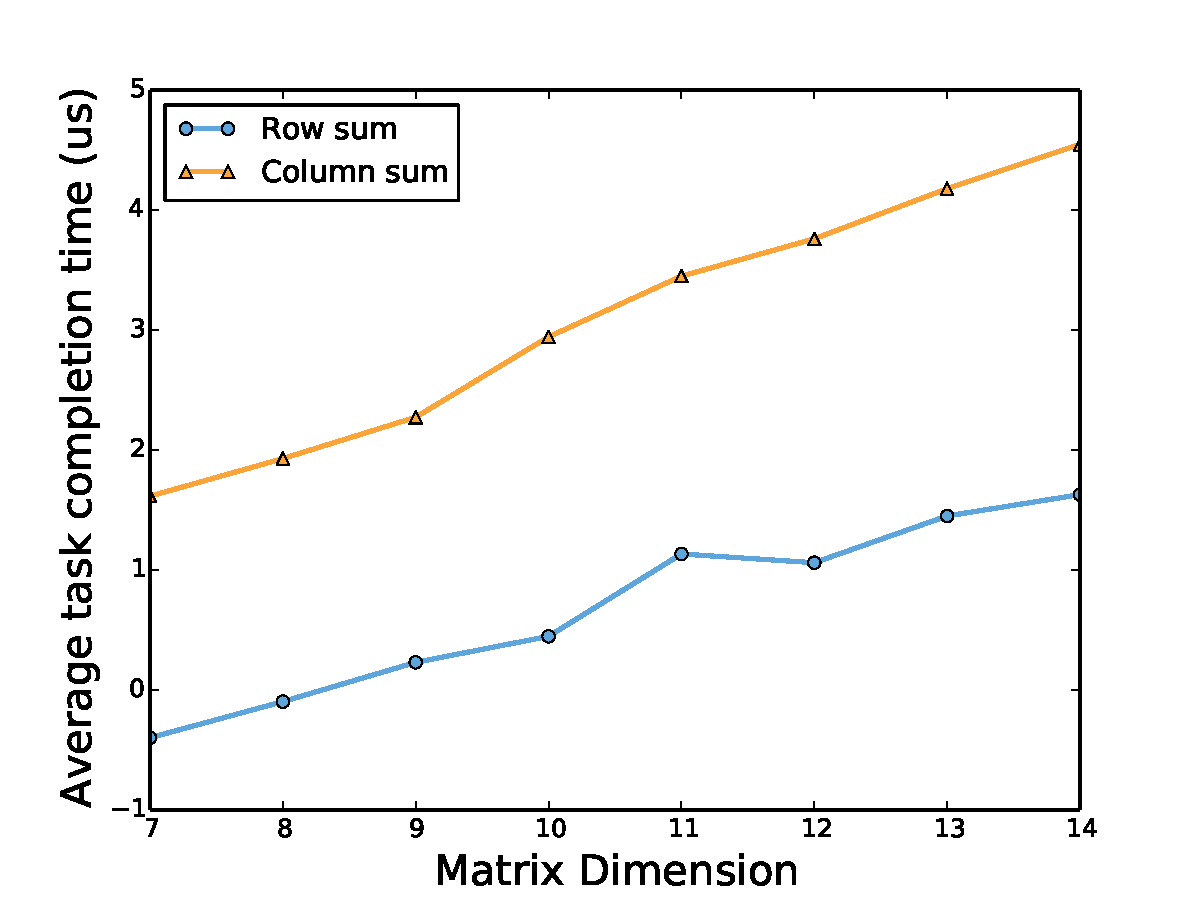
\includegraphics[scale=0.35]{images/rowmajor}
	\caption{Performance comparison of row and column oriented access patterns.
	The dimension attribute along the x-axis refers to the $\log_2$ of
	the length of the two-dimensional square matrix. }
	\label{fig:perf}
\end{figure*}

\subsection{The Problem}

In this work, we focus on applications that have complex workloads with
mixed DRAM access patterns. For instance, in a hybrid transaction and
analytical processing (HTAP) workload~\cite{grund10}, the DBMS needs to
access both the tuples and columns of a table efficiently. Irrespective of
whether the DBMS uses a pure-row or pure-columnar layout, one of the two
access patterns has to suffer from poor DRAM performance. For instance, assume
that the DBMS uses a pure-row layout and that the size of each tuple is one
cacheline (64 bytes).
When serving an analytical query that needs to sum up the values in a
particular column, we need to access only that part of the tuple
in all the tuples in the table.
This means that we would like to access only part of a cacheline.
This is however not feasible in current hardware, as the data is laid
out in tuple-major order.

In future hardware systems, we anticipate that we will have new DRAM access
primitives that allow us to access parts of a cacheline and not just
entire cachelines.
These primitives will allow the application to read a cacheline
composed of data stored in different DRAM rows by specifying
an DRAM \textit{access pattern}. This is illustrated in ~\cref{fig:primitives}.
Consider a 4$\times$4 toy matrix. In the default row-major layout,
fetching the first column will require four DRAM read operations as
they will be serialized at the same bank. If we \textit{shuffle}
the tile to DRAM row mapping as shown below, we observe that we can
access both the first row (cacheline 1) and first column (denoted by, say,
cacheline 1.2) using a single DRAM read operation.
This effectively allows us to retrieve the required data (for instance, a column
in a matrix) in fewer DRAM operations compared to existing DRAM access primitives.
Therefore, we can achieve (1) lower DRAM latency, (2) more efficient DRAM
bandwidth utilization, and (3) lower energy consumption.

\begin{figure*}[ht]
	\centering
	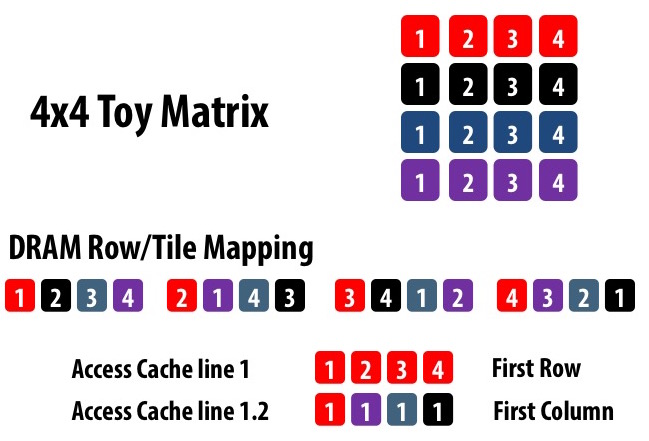
\includegraphics[width=0.8\textwidth]{images/primitives}
	\caption{Novel DRAM access primitives that allow the application to read
	both a column or a row in a small matrix in a single DRAM read operation.}
	\label{fig:primitives}
\end{figure*}


The problem we address in this work involves designing a compiler pass that
allows us to \textit{automatically} identify the application's access
patterns and transforms the program to make use of these novel DRAM access
primitives.
This reduces the burden on the programmer and thereby simplifies the adoption
of these DRAM access primitives.
At a high level, this involves addressing two subproblems:

\begin{itemize}
  \item {Figuring out the different application access patterns}
  \item {Mapping the access patterns to make use of underlying DRAM access primitives.}
\end{itemize}

\subsection{Our Approach}

We have implemented an LLVM compiler pass that analyses data structure access patterns.
Currently, this targets multi-dimensional arrays of primitive data types as well as structures.
We assume that the programmer has annotated the data structures that should be
analysed using LLVM annotations.
We could apply the analysis on all loads and stores, but we wanted to restrict our
analysis to important data structures that are accessed several times in loops.
In the first stage of the pass, we parse the annotations to determine these data structures.
Then, for each loop within a function, we analyze loads and stores to these
data structures using LLVM's Scalar Evolution (SCEV) pass. Given a scope and a
register, the SCEV pass yields an expression that represents the register's
evolution inside the scope. When applied to the load or store address of the
annotated data structure in the innermost loop, this gives us the stride
with which the program performs these loads and stores.

\subsection{Related Work}

-

\subsection{Contributions}

We make the following contributions in this project:

\begin{itemize}
  \item {We implemented an LLVM pass that determines the different data
  structure access patterns by an application.}
  \item {We developed a basic DRAM access cost model that allows the compiler to
  map the application access pattern to the most optimal DRAM access pattern.}
  \item {We illustrate the performance benefits of these novel DRAM access primitive
  through a quantitative evaluation on different workloads in a custom matrix
  library.}
\end{itemize}

\section{Matrix Access Pattern Analysis}

The goal of this analysis is to identify the different application access
patterns and then map then onto an efficient DRAM access primitive to improve
cache and memory subsystem performance. In this section, we will first present
the compiler pass and then describe the DRAM access cost model that we leverage
in our mapping function.

\subsection{LLVM Pass}

We define an application's data structure access pattern in terms of two 
parameters : (1) \textit{stride}, and (2) \textit{offset}. 
For instance, consider an array of structures, each of which contains two
integer fields. 
Then, if the application accesses the second field in all the structures 
in the array in a loop, we denote that access pattern as $\{4,+,8\}$. 
Here, the first member is the offset and the second element is the stride.

We implemented a compiler pass that analyses our matrix library automatically
to determine the stride and offset of the application's access patterns.
We assume that the programmer annotates the data structures that should
be analysed using LLVM annotations.
In theory, we can apply our analysis on all loads and stores in the program.
However, we wanted to restrict our analysis to important data structures
as that approach is more practical.
Further, we also focus only on memory accesses within \textit{loops} in the 
application. This is because we believe that optimizing these memory accesses
with the novel DRAM access primitives will be sufficient to realize
significant application speedups.

This compiler pass consists of three stages :
\begin{itemize}
  \item{We first parse the programmer annotations to determine the critical data
  structures.}
  \item{Then, for each loop in the program, we analyze the loads and
  stores associated with these data structures to determine the access pattern.}
  \item{Finally, we use the cost model to map the access pattern to the
  relevant DRAM access primitive.}
\end{itemize}

We implemented the first stage using LLVM's support for data member annotations.
Then, we leveraged the scalar evolution (SCEV) analysis~\cite{llvm15} functions
in the second stage of the compiler pass.
These functions support the analysis of scalar expressions within loops and
help recognize general induction variables.
Given a program \textit{scope} and a register, we can use these functions to
obtain an expression that represents the register's evolution inside the scope.
We applied these functions to the load and store addresses of the annotated 
data structure within the scope of the innermost loop. We then parsed the
recursive expression and delinearized it to obtain the stride and offset
with which the application accesses the critical data structures in the loop.

The output of the compiler pass on a sample program is shown below :

\begin{lstlisting}[caption={Sample Input Program},label={lst:input}]

------------------------------------------------------------
INPUT PROGRAM
------------------------------------------------------------

void foo(long n, long m)  {
  __attribute__((annotate(``this is important''))) int A[n][m];
  
  struct key{
    char a;
    char b;
    char c;
  };
  __attribute__((annotate(``critical''))) struct key keys[100];

  char x;
  for (long i = 0; i < n; i++) {
    for (long j = 0; j < m; j++){
      A[i][j] = 0;
      A[j][i] = 0;
      x = keys[i].a;
      keys[i].b = x;
    }
  }
}
\end{lstlisting}

\begin{lstlisting}[caption={Analysis Output},label={lst:output}]

------------------------------------------------------------
ANALYSIS OUTPUT :
------------------------------------------------------------


Analysing function :: foo:

------------------------------
Annotations found :
------------------------------

tests/a.c:i32 5           
%vla = alloca i32, i32 %1, align 4    
this is important

tests/a.c:i32 13          
%keys = alloca [100 x %struct.key], align 1   
critical

------------------------------
Loads/Stores :
------------------------------

------------------------------
Instruction:   store i32 0, i32* %arrayidx6, align 4
------------------------------

Access Pattern :
{{0,+,(4 * %m)}<%for.cond>,+,4}<nw><%for.cond3>

Delinearized Access Pattern :
[{0,+,1}<nuw><nsw><%for.cond>][{0,+,1}<nuw><nsw><%for.cond3>]

------------------------------
Instruction:   store i32 0, i32* %arrayidx8, align 4
------------------------------

Access Pattern :
{{0,+,4}<nuw><nsw><%for.cond>,+,(4 * %m)}<%for.cond3>

Delinearized Access Pattern :
[{0,+,1}<nuw><nsw><%for.cond3>][{0,+,1}<nuw><nsw><%for.cond>]

------------------------------
Instruction:   %4 = load i8* %a, align 1
------------------------------

Access Pattern :
{0,+,3}<nuw><nsw><%for.cond>

------------------------------
Instruction:   store i8 %4, i8* %b, align 1
------------------------------

Access Pattern :
{1,+,3}<nw><%for.cond>

\end{lstlisting}

In the listing above, we observe that our pass can handle multi-dimensional
arrays of both primitive and aggregate data types. It can clearly distinguish
the row-oriented and colum-oriented access patterns \texttt{A[i][j]} and 
\texttt{A[j][i]}. In the former case, the access pattern is of the form :\\
  
\texttt{\{\{0,+,(4 * \%m)\}<\%for.cond>,+,4\}<nw><\%for.cond3>},\\

i.e. the accesses are row-oriented. In the latter case, the stride is larger and
the accesses are column-oriented. This is even more evident from the delinearized access
patterns, wherein the order of the for-loop conditions are inverted in the
two cases.

Similary, in the case of the array of structures, the offset of the first
and second character fields within the structure are distinguished. This is
evident in the \texttt{\{0,+,3\}<nuw><nsw><\%for.cond>} and
\texttt{\{1,+,3\}<nw><\%for.cond>} access patterns. 
We have successfully tested our compiler pass on more complex access patterns. 
Overall, we can effectively analyze the loads and stores associated with the
critical data structures using the pass.

\subsection{DRAM Access Cost Model}

\begin{figure*}[ht!]
	\centering
	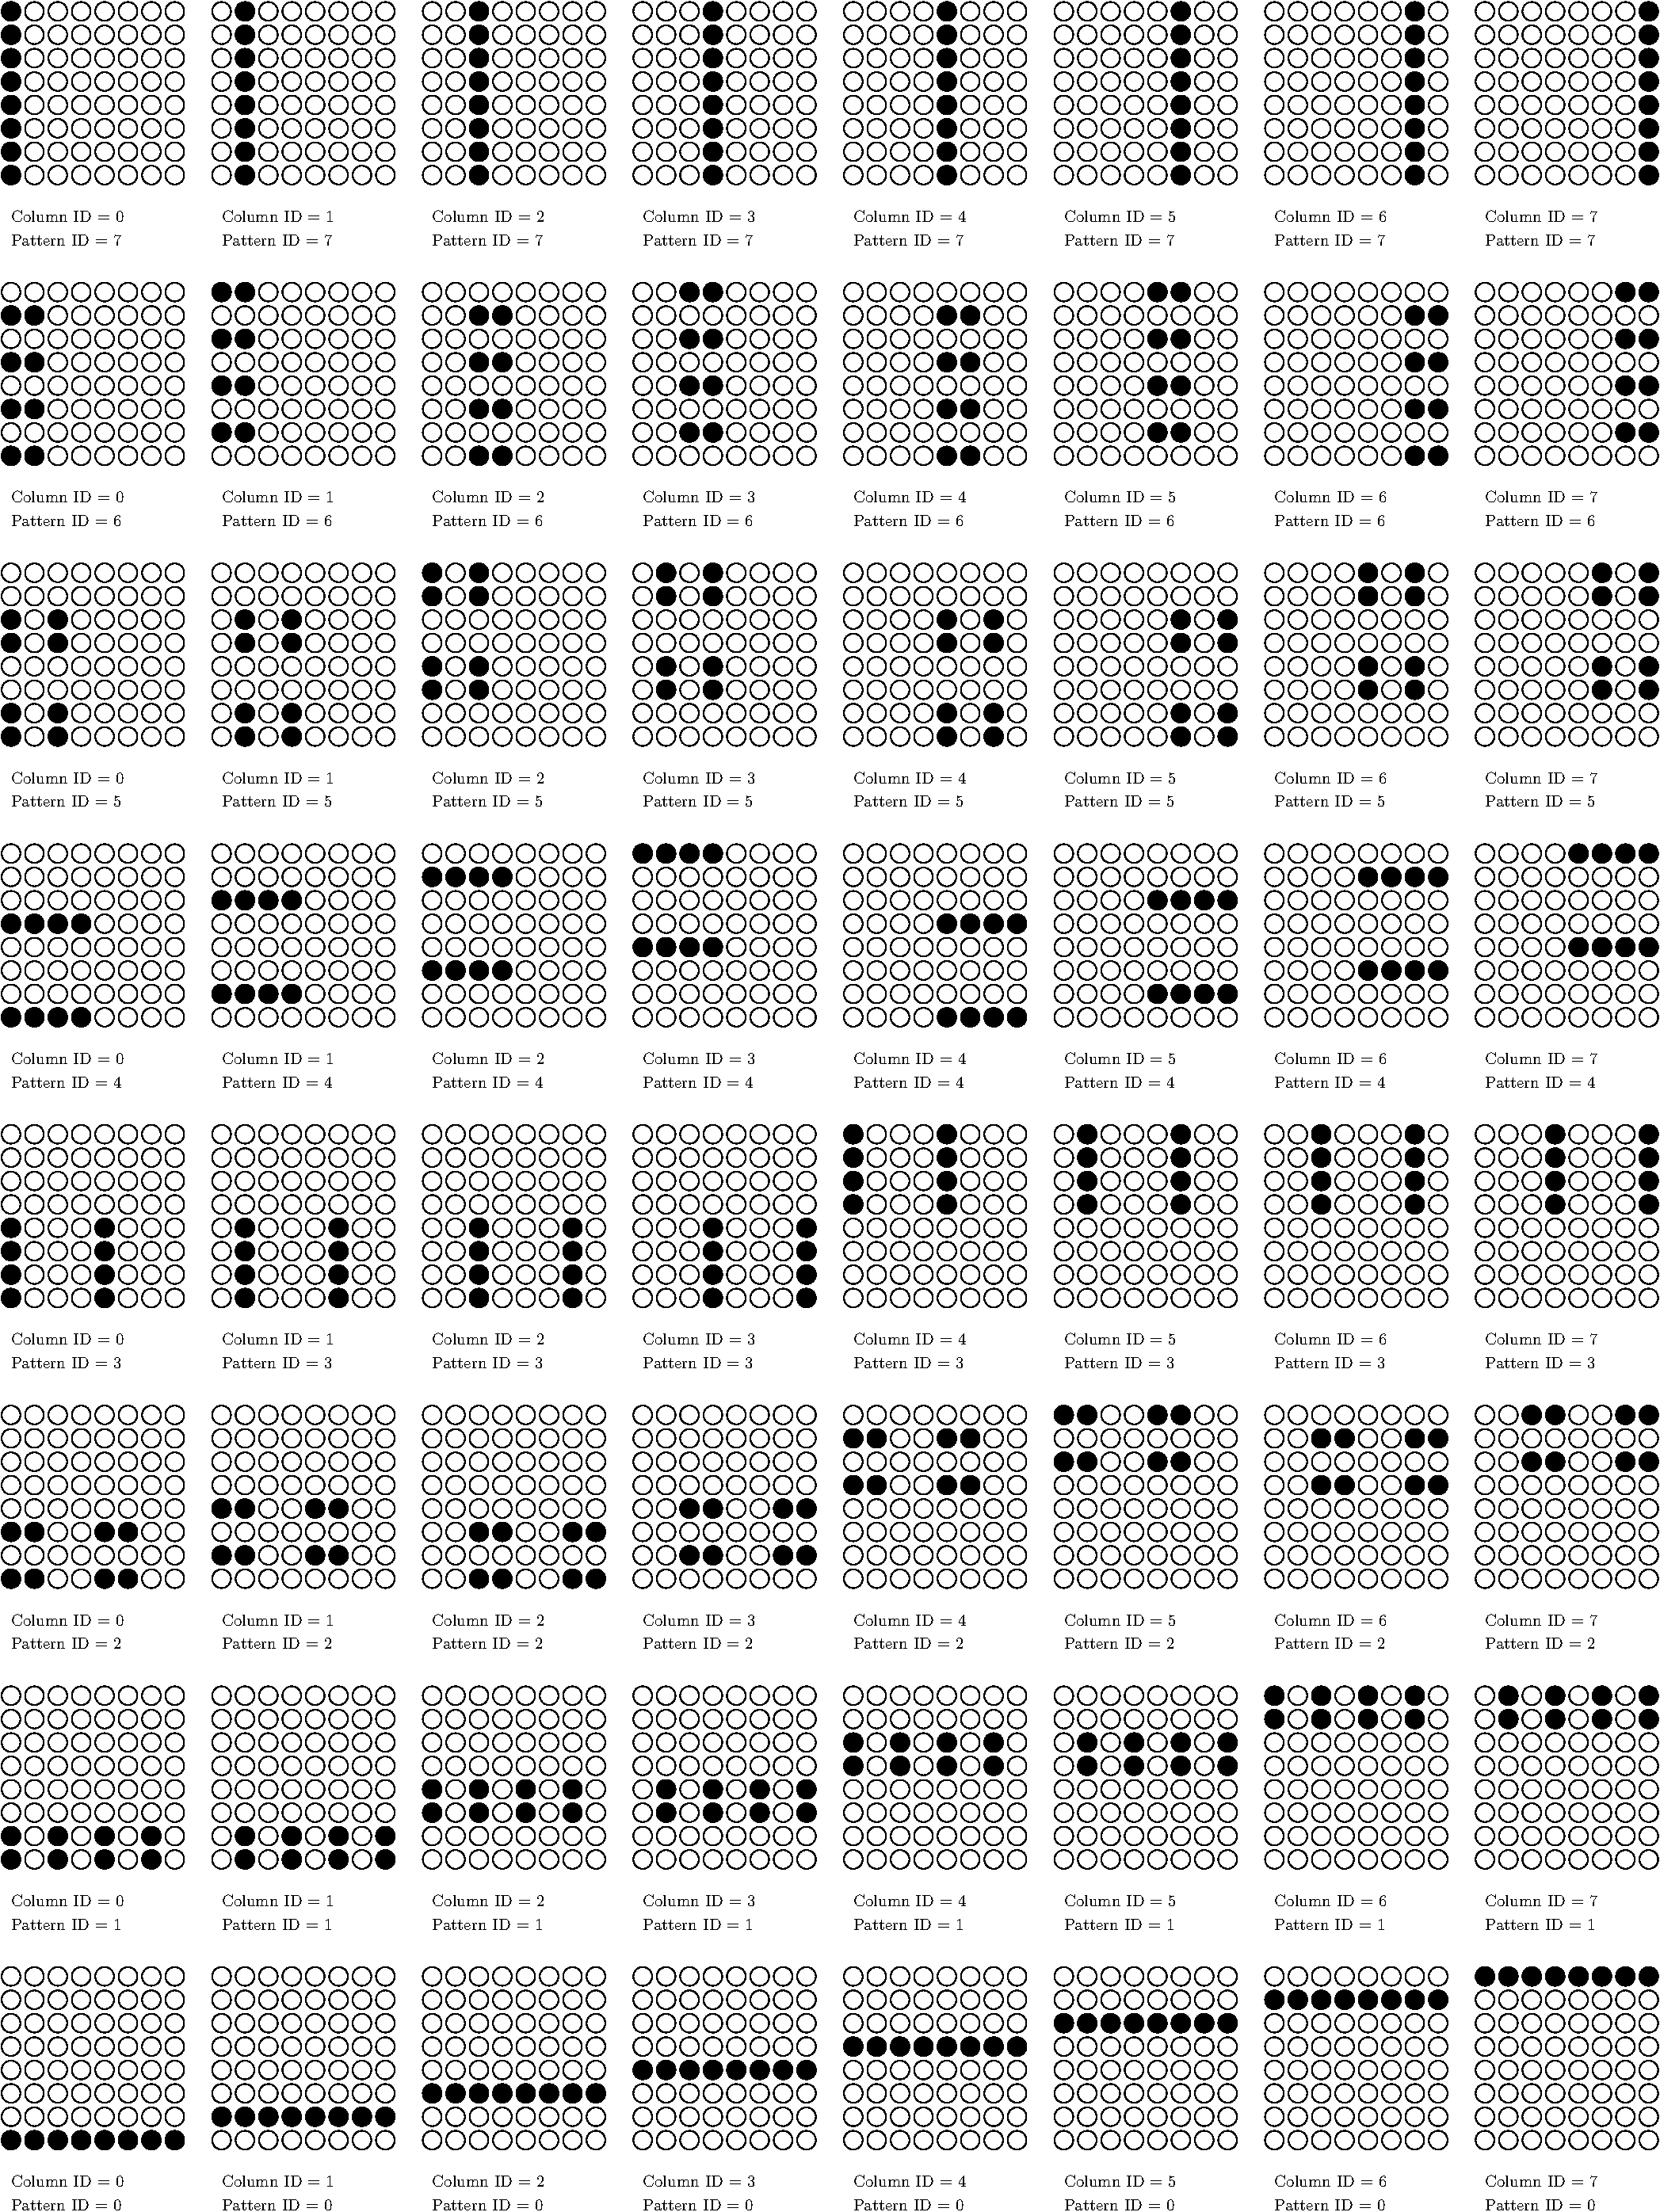
\includegraphics[width=0.9\textwidth]{images/pattern}
	\caption{List of possible patterns for a 8$\times$8 matrix with a given
	shuffling function. The column id refers to the cacheline being accessed. 
	The elements of the cacheline that are highlighted are returned to the
	application.}
	\label{fig:pattern}
\end{figure*}

We now describe the cost model we developed to help us map the
application's access patterns to the relevant DRAM access primitive.
To begin with, consider the list of possible patterns for 8$\times$8 
toy matrix with a given shuffling function shown in~\cref{fig:pattern}. 
We observe that there are $64$ total DRAM access patterns. 
In each case, the \textit{column id} refers to the cacheline being accessed,
while the \textit{pattern id} is the auxiliary information that we can 
supply using the novel DRAM access primitives.

The elements of the cacheline that are highlighted will be returned to the 
application that is requesting the desired cacheline and pattern id.
We first note that using this tile to DRAM row mapping, we can access both
the first row and first column in the matrix in a single DRAM read operation.


\section{Experimental Setup}

To evaluate the effectiveness of our approach, we measure the runtime performance of the application utilizing new DRAM acces primitives using a prototype.

\begin{itemize}

  \item \textbf{Compiler Pass:} We implemented an LLVM 3.5 compiler pass that analyses data structure access patterns. We utilize programmer annotation support to pin-point the data structrues that we wish to analyze, and make use of Scalar Evolution (SCEV) pass provided by LLVM framework to examine the access indices. We then cross reference the result with available patterns from DRAM primitives \ref{fig:pattern} to compute the pattern id that maximizes the performance.
  \item \textbf{Gem 5:} Gem5 simulator is a configurable simulation framework that can emulate novel DRAM access primitives. We use modified version of Gem5, that takes in pattern id from unused address bits from the prefetch instruction and emulates the access pattern. However, due to functional limitations we were not to obtain the statistics we needed for the evaluation and we decided to measure performance directly using sets of test applications.
\end{itemize}

\begin{table}[t]
    \centering
    \begin{tabular}{c|c}
  \textbf{CPU} & \\
    \textbf{RAM} & \\
    \textbf{HDD} & \\

  \end{tabular}
    \caption{
        \textbf{System Specification} --
        The specification of the system used for evaluation
    }
    \label{tab:spec}
\end{table}

\section{Experimental Evaluation}

We evaluate effectiveness of the new architecture by comparing the performance with and without
the support from DRAM for new access primitives. Specifically, we compare the performance
of row major access pattern and other access patterns implemented in a system without the support,
as we assume that performance behavior of new patterns will be similar to regular row major
access pattern. We use following test code for the evaluation:

\begin{Verbatim}[fontsize=\small]
void test(void * matrix, int pattern_id, int rd_wr_ratio, int scale) {
    StartTimer();
    for(k = 0 ; k < repeat; k++) {
        AccessMatrix(mat, pattern_id, rd_wr_ratio, scale);
    }
    StopTimer();
}
\end{Verbatim}


We report the runtime of the test case as we vary the pattern
(\textit{pattern\_id}), read write ratio(\textit{rd\_wr\_ratio}) and size of the tile (\textit{scale}).

\begin{itemize}
  \item \textbf{Pattern} We implemented all access patterns depicted in \ref{fig:pattern} in C.
  \item \textbf{Workload} We define the four workloads (Read only, Read heavy,
Balanced, Write Heavy) using a parameter, read write ratio (0, 0.25, 0.5, 0.75 respectively).
\textit{AccessMatrix} function randomly reads or writes different tiles of the matrix and read
write ratio defines proportion of reads and writes in the generated workload.
  \item \textbf{Tile size} This is the dimension of the pattern matrix. We evaluated the
  workload using dimension 64, 128, 256, 512.
\end{itemize}

We summarize our main result in Figure~\ref{fig:evaluation}, where we report the normalized runtime
with respect to the baseline (row major) pattern \textit{P0}. Among all patterns, we expect for P 7 (Columnar access) to perform most poorly as incurs most cache miss in the current architecture. 

 We observe that in general, all other patterns
perform poorly in comparison to the baseline pattern. This is in line with our expectation, 
as the memory architecture is optimized for row major access pattern and any access besides row major pattern will introduce one or more cache misses. 

Furthermore, we observe that the performance degrades as the workload contains more store operations. 
This effect is also expected as more write instructions 
increase the number of modifications to the content of the 
memory. This will provide more opportunity for optimization under new acces primitives. 

Finally we also analyze the effect of the tile size. We observe that the effects of access primites are more
significant as we increase the tile size. This effect is more drastic for pattern 7 where the dimension of the
tile is directly related to number of cache misses. 


\begin{figure*}[t]
    \centering
    \subfloat[64$\times$64 tiles]{
	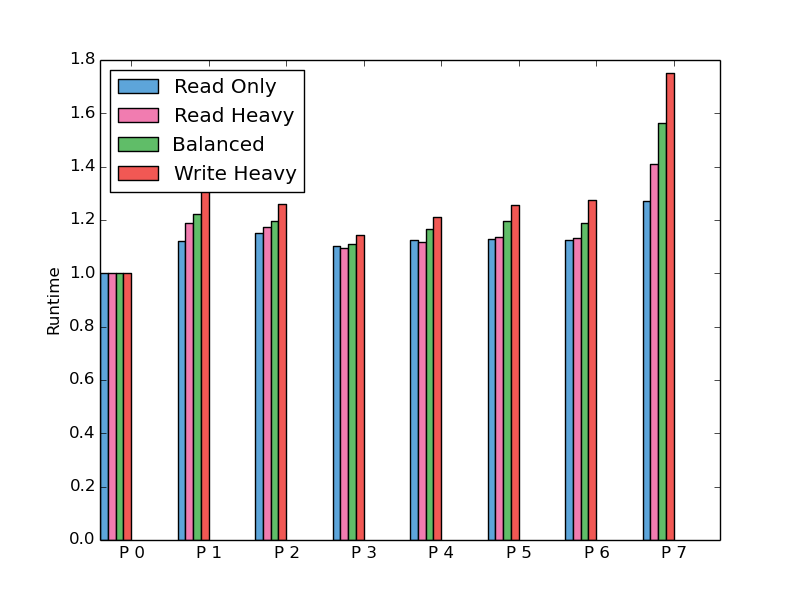
\includegraphics[width=0.5\textwidth]{images/64_runtime}
    }
    \subfloat[128$\times$128 tiless]{
	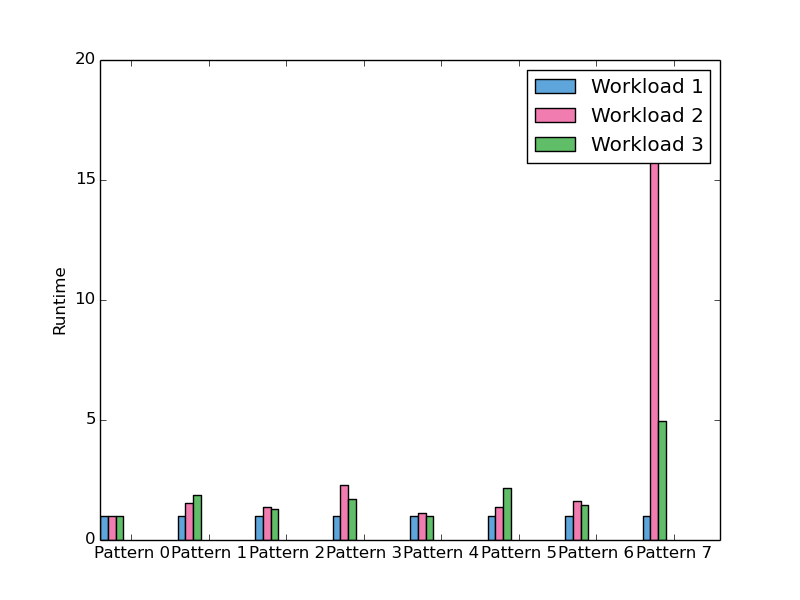
\includegraphics[width=0.5\textwidth]{images/128_runtime}
    }\\
    \subfloat[256$\times$256 tiles]{
	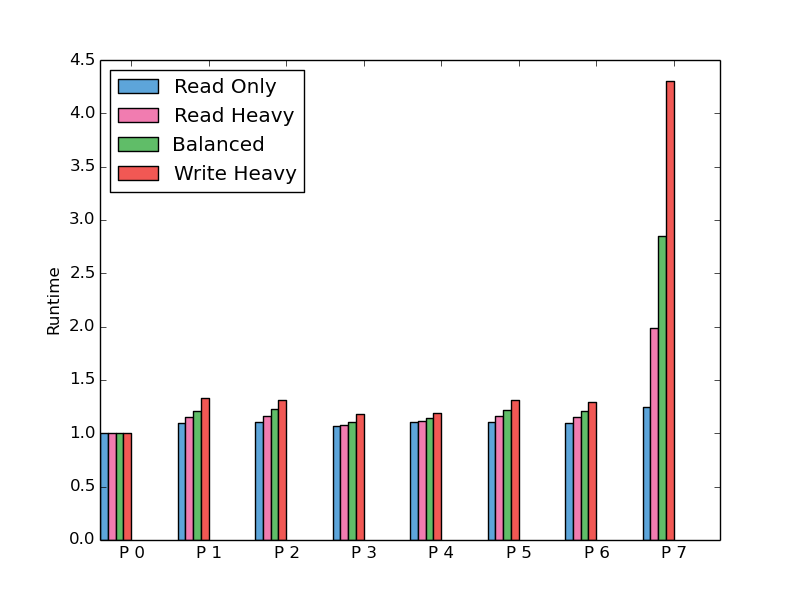
\includegraphics[width=0.5\textwidth]{images/256_runtime}
    }
    \subfloat[512$\times$512 tiless]{
	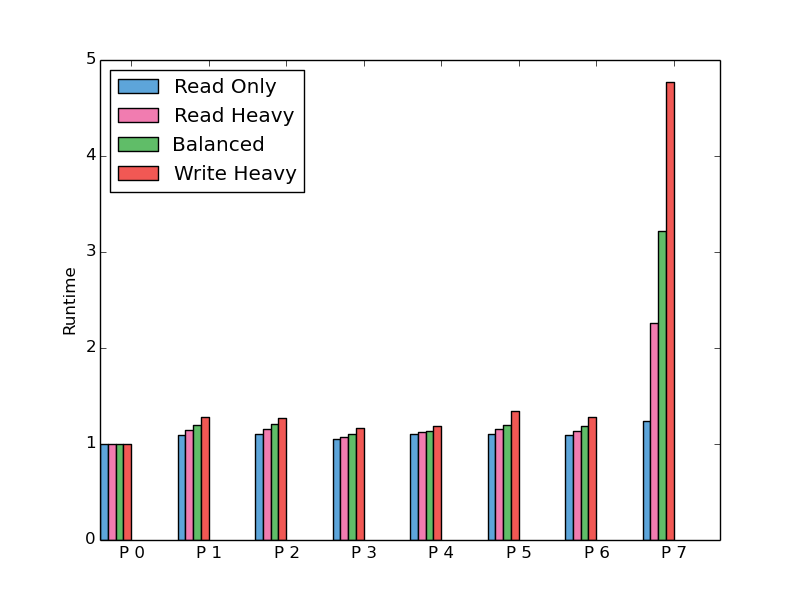
\includegraphics[width=0.5\textwidth]{images/512_runtime}
    }
    \caption{\textbf{Performance -- Evaluation of workload}}

    \label{fig:evaluation}
\end{figure*}

\section{Surprises and Lessons Learned}
We were pleasantly surprised by the support in LLVM for analysing scalar expressions and annotations.
This helped reduce the complexity of the compiler pass.

\section{Conclusions and Future Work}

We present the compiler support for new memory architecture that provides new types of access primitives. We discussed the potential benefits and evaluated the runtime performance as we vary factors (pattern type, workload, and tile size) that affects the performance. We show that the new types of access can provide up to 5x speed up in run time. 

As discuss in the report, we restrict attention to the pre-defined patterns and synthetic low level array access workload. More extensive evaluation against the realistic workload may provide more detailed analysis of the performance behavior and may pose interesting challenge for future work. 


\section{Distribution of Total Credit}

\bibliographystyle{acm}
\bibliography{ref}

\end{document}

%%% Local Variables:
%%% mode: latex
%%% TeX-master: "."
%%% End:
